\documentclass[11pt]{article}
\usepackage[french]{babel}

\usepackage[utf8]{inputenc}
\usepackage{palatino}
\usepackage[T1]{fontenc}


\usepackage{url}
\usepackage{amsmath}

\usepackage[top=2cm,bottom=2cm,left=2.1cm,right=2.1cm,headsep=10pt,a4paper]{geometry}
\usepackage{fancyhdr}


\usepackage{graphicx,float} % figure et placement de figure
\usepackage{listings} %%inclusion de programmes

\lstset{
language=C,
basicstyle=\ttfamily\small, %
identifierstyle=\color{black}, %
keywordstyle=\color{blue}, %
stringstyle=\color{blue}, %
commentstyle=\it\color{green}, %
}

\usepackage{xcolor}

\pagestyle{fancy}
\lhead{}
\chead{\fontsize{10}{10}{Mif20 - UCBL - 2013/2014}}
\rhead{\thepage}
\lfoot{\fontsize{10}{10}{Rapport de TER de Aurélien CHEMIER}}

\renewcommand{\headrulewidth}{0pt}
\renewcommand{\footrulewidth}{0pt}


 \author{\fontsize{14}{14}{\bf Aurélien CHEMIER}}
 \title{\fontsize{16}{16}{{\bf Rapport de TER: Analyse de pointeur dans LLVM}}}
 \date{\fontsize{11}{11}{Janvier-Février 2014}}

\begin{document}

\thispagestyle{empty}
\maketitle

\begin{abstract}
  Les optimisations réalisées à l'intérieur d'un compilateur, pour
  améliorer l'efficacité du code généré, ont besoin d'informations
  détectées statiquement (taille des tableaux, variables constantes,
  etc).  Certaines de ces analyses très utiles, ne fonctionnent que
  dans des cas "syntaxiquement simples". L'objectif de ce TER est
  d'améliorer le domaine d'application des optimisations de tableaux
  réalisées dans l'équipe Compsys. En effet, ces optimisations sont
  pour le moment restreintes à des tableaux de taille statique, et à
  des programmes qui ne contiennent aucune utilisation de pointeurs.

 \par Or, on constate souvent que les pointeurs ne sont utilisés en C
 que de façon rudimentaire : transmission d'arguments par adresses,
 allocation dynamique de tableau réalisée une unique fois,
 descripteurs de tableaux, pseudo-indices.
  
  \par L'objectif est donc de réaliser un outil de détection de ces
  usages simples et de transformer  le programme initial en un
  programme \textit{sémantiquement} équivalent qu'on pourra ensuite
  optimiser en utilisant les outils de l'équipe.\\
  \textbf{Mots clefs}:  Optimisation, pointeurs, C
\end{abstract}


\tableofcontents


\newpage
\section{Introduction}
  L'avancée technologique des plateformes matérielles, avec des caractéristiques toujours plus complexes, 
  rend nécessaire des analyses toujours plus fines du code source, que ce soit pour des buts 
  d'optimisation à la compilation (optimisation de taille mémoire, de l'usage du cache...) ou d'optimisations lors de l'exécution.
  
  COMPSYS est une équipe-projet de recherche commune à Inria et au Laboratoire de l'Informatique du Parallélisme (LIP).
  Elle est localisée à l'Ecole Normale Supérieure de Lyon (ENS Lyon).
  L'objectif de Compsys est le développement de techniques de compilation, plus précisément d'optimisations de codes, 
  appliquées aux domaine des systèmes embarqués de calcul (\emph{embedded computing systems}).
  

%%non, on ne veut pas optimiser les pointeurs, on n'optimise rien en
%%faisant ça.

  Les optimisations de code réalisées dans l'équipe Compsys
  s'effectuent pour la plupart au niveau des parcours de tableaux
  (optimisations dites \emph{polyédriques}). Elles ont pour but de
  favoriser le parallélisme, la localité (pour éviter les défauts
  de cache), et d'optimiser les chargement de données. Cependant,
  pour des raisons de simplicité, les optimisations ne sont pour
  l'instant appliquées qu'à des programmes sans pointeurs, et dans
  lequel les tableaux sont déclarés statiquement.

  Or, dans un programme C, l'utilisation  des pointeurs est
  souvent basique (tableau dynamique, ...). 
  En reconnaissant certaines utilisations simples de pointeurs
  dans les programmes , il sera possible de modifier le code pour
  utiliser les optimisations déjà écrites. 

  
  Durant son stage de L3, Christophe Bacara a démarré une
  implémentation d'outils et d'algorithmes permettant de
  caractériser les utilisations de pointeur d'un 
  code C donné. Il utilise pour cela le \emph{framework} Clang/LLVM.
  Le
  résultat\footnote{\url{http://laure.gonnord.org/pro/papers/rapportBacara.pdf}}
  est un stockage dans une structure de données d'un certain
  nombre d'informations concernant les pointeurs du programme   (pointeurs constants, pointeurs "cachant" des tableaux).
  
 
  L'objectif du TER était donc d'utiliser les informations
  statiquement récupérées dans le programme C pour transformer ce code
  C en un programme équivalent. Ce TER a été encadré par Laure Gonnord.
  
\section{Analyse Statique de code avec LLVM/Clang}

  \subsection{Le framework LLVM/Clang}
  
    Le projet LLVM3 est né en 2000 à l’Université de l’Illinois, sous la direction
    de Chris Lattner et Vikram Adve. Il s’agit d’une infrastructure de compilateur,
    fondée sur une représentation intermédiaire du code, de type
    SSA (\emph{single static assignment},
    conçue pour l’optimisation d’un programme à tous les niveaux
    (analyse, compilation,
    édition de liens, exécution). LLVM est composé de librairies qui permettent
    de manipuler cette représentation du code. A l’origine, l’implémentation concernait les
    langages C et C++, mais il existe désormais une grande variétés de frontend\footnote{Passes de compilation qui effectuent l’analyse lexicale et syntaxique de la source
    en entrée afin de la transformer en représentation intermédiaire, nécessaire à la suite du
    processus de compilation (optimisation, édition de liens, ...)} 
    : Ruby, Python,Java, PHP, et Fortran, parmi d’autres.
    LLVM contient nombre d’optimisations, ainsi que des générateurs de code
    pour de nombreux processeurs. LLVM est diffusé sous licence University Of
    Illinois Open Source, licence de type BSD. LLVM est codé en C++.

    Clang (codé en C++) et est le front-end de LLVM. C’est celui qui
    est chargé de faire les analyses lexicales et syntaxiques, de construire l’arbre
    de syntaxe abstrait du programme, et de le convertir en code intermédiaire,
    compréhensible par LLVM.
    
  \subsection{Représentation des instructions dans LLVM/Clang}

    Clang utilise une hiérarchie de classes pour représenter les différentes
    instructions rencontrées dans un programme. \emph{Stmt} est la super-classe de
    cette hiérarchie, et représente de manière abstraite n'importe quelle
    instruction. Une partie de cette architecture est présentée dans la
    figure~\ref{fig:graph}

    \begin{figure}[H]
      \centering
      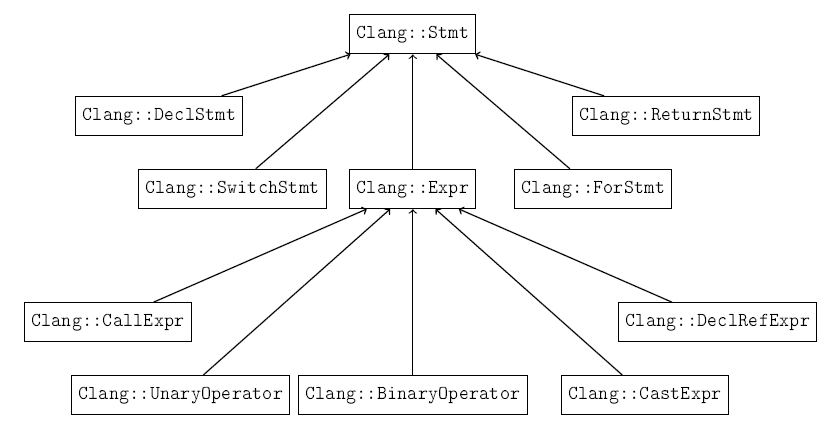
\includegraphics[scale=0.7]{soluce/graph.jpg} 
      \caption{Partie de l'architecture de Clang}
      \label{fig:graph}
    \end{figure}

    \medskip
    De plus, \emph{Stmt}, ainsi que toutes les classes qui en héritent, se comporte
    comme un conteneur. Elle peut donc stocker des pointeurs vers des objets enfants
    de type \emph{Stmt} (et donc, par polymorphisme\footnote{Principe de
    programmation orientée objet, qui considère qu'un objet d'une classe B, héritant
    d'une classe A, peut-être considéré comme une extension de la classe A, et peut
    donc être manipulé comme un objet de classe A.}, de n'importe quelle classe
    héritant de \emph{Stmt}). Ainsi, en itérant sur un objet de type
    \emph{Stmt}, il est possible de récupérer l'ensemble des sous-instructions
    contenues dans cet objet. Un exemple de représentation d'une instruction est
    disponible avec la figure~\ref{fig:exemple}.

    \begin{figure}[H]
      \centering
      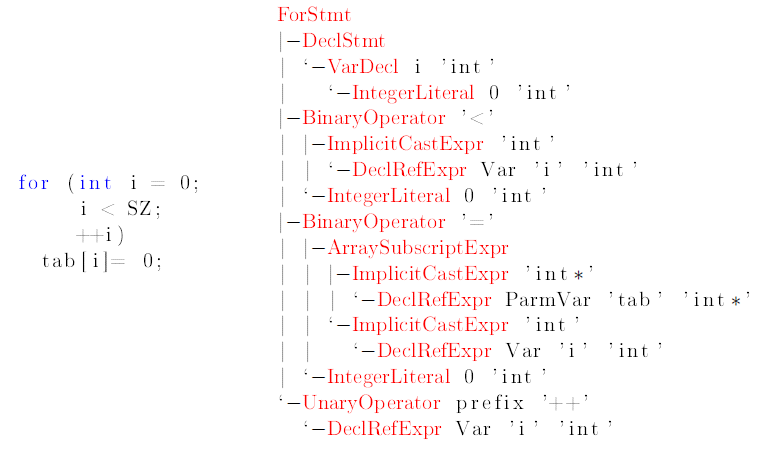
\includegraphics[scale=0.7]{soluce/exemple.jpg} 
      \caption{Représentation d'une instruction étudié par Clang}
      \label{fig:exemple}
    \end{figure}

  \subsection{Travail existant}

    Le travail de C. Bacara m'a permis d'avoir à ma disposition différents outils pour l'étude des pointeurs dans un code C.

    \begin{itemize}
      \item La fabrication et le parcours du CFG (Graphe de flot de
        contrôle, voir figure \ref{fig:CFG} par exemple) du code à optimiser.
      \item Les pointeurs constants: c'est à dire les pointeurs dont la valeur ne change pas dans la fonction étudié.
      Pour celà, il faut parcourir le CFG, une fois celui-ci créé, et contrôler la non-modification de la valeur des pointeurs.
      \item Les alias de pointeurs: c'est à dire lorsque plusieurs pointeurs désignent le même objet.
      
      Pour stocker les informations d'alias et de pointeur constant,
      Christophe Bacara a utilisé une structure donnée faisant appel à
      un codage matriciel (qui lui permet de coder le graphe orienté de la relation ``pointe sur'').
      
      Par exemple pour le code suivant:
      
      \lstinputlisting[caption={Code exemple pour les matrices d'alias},language=C,frame=single]{Exemple/alias.c}
      
      L'analyseur créera d'abord une matrice carré avec les pointeurs et les cibles pointés. Les lignes indiquent les pointeurs et les colonnes les cibles.\\
      \label{alias}
     \begin{math}
      \begin{pmatrix}
	1 & 0 & 0 &  0 \\
	0 & 1 & 0 & 0 \\
	0 & 1 & 1 & 0  \\
	0 & 1 & 0 & 1 
      \end{pmatrix}
     \end{math}
     \\
     
    Ensuite, on créé la matrice symétrique de la matrice précédente. En effet dans l'exemple, on a le pointeur \textit{p3} qui pointe sur \textit{p2},
    donc, si on connaît \textit{p2}, on connaît également \textit{p3}.\\
    
    \begin{math}
      \begin{pmatrix}
	1 & 0 & 0 & 0 \\
	0 & 1 & 1 & 1 \\
	0 & 1 & 1 & 0  \\
	0 & 1 & 0 & 1 
      \end{pmatrix}
     \end{math}
     \\
    
    Dernière étape, il faut prendre en compte les pointeurs qui pointent sur une même cible (a pointe sur b, c pointe sur b...)
    et les suites de pointeurs . (a pointe sur b qui pointe sur c
    ...). Une clôture transitive est donc implémentée~:\\
    
    \begin{math}
      \begin{pmatrix}
	1 & 0 & 0 & 0 \\
	0 & 1 & 1 & 1 \\
	0 & 1 & 1 & 1  \\
	0 & 1 & 1 & 1 
      \end{pmatrix}
     \end{math}
     \\
    
    Ainsi avec cette matrice, on connaît tous les alias du code.
    \end{itemize}
      
    
  \subsection{Critiques à l'utilisation de Clang}
    La librairie Clang permet de parser le code C étudié et d'obtenir
    à la fois l'arbre de syntaxe abstraite (AST) et le  graphe de flot
    de contrôle (CFG).

    Une fois qu'on dispose de l'AST/CFG, il est facile  de vérifier
    l'utilisation faite des pointeurs. Et donc de manière générale,
    d'obtenir des informations statiques sur les constructions
    syntaxiques du programme, ce qui est fait par le code existant de
    C. Bacara.

    Dans la suite, ce que l'on désire faire est une modification de
    cette structure d'AST ou de CFG, par exemple en remplacement un
    \emph{statement} (affectation, test, \ldots) par un autre. Il
    faudra donc modifier cette structure interne. La librairie Clang
    fournit des fonctions génériques de parcours, mais pas des
    fonctions de modification (en tout cas pas au même niveau
    d'utilisation). La modification sera donc plus complexe que la
    recherche d'information.



% , et de là optimiser le code (ou
%     en tout cas modifier l'AST

%     Dans LLVM, le parcours de l'AST est caché. 
%     C'est pratique si l'on travaille sur une fonction spécifique mais celà devient compliqué si l'on travaille globalement.

\section{Transformation source à source à sémantique constante}

  \subsection{Rappel du problème}

    L'objectif du TER est de trouver certaines utilisations
    spécifiques des pointeurs dans le but de les optimiser.  Dans
    cette partie nous analysons les différentes transformations
    simples que nous désirons réaliser.


    
    \subsubsection{Exemple 1: pointeur constant sur variable}
      Cet exemple traite de l'optimisation dans le cas d'un pointeur constant.
      
      \lstinputlisting[caption={Exemple de pointeur constant},language=C,frame=single]{Exemple/pointeurConstant.c}
      
      Dans cet exemple, on voit bien que le pointeur \textit{p} est un alias de \textit{a}. 
      Quand on modifie la valeur pointé par \textit{p}, \textit{a} est modifié et réciproquement.
      
      Le travail d'optimisation consiste à voir que le pointeur \textit{p} est constant et qu'il est un alias de \textit{a}. 
      Et de là, on remplace toutes les occurences de \textit{p} par \textit{a}.
      
      Avec le travail déjà effectué, on peut récupérer le fait que \textit{p} est un alias \textit{a} et il suffit de modifier le rewriter pour appliquer l'optimisation.
      
      \lstinputlisting[caption={ Optimisation de l'exemple précédent},language=C,frame=single]{Exemple/pointeurConstantOpt.c}
    
    \subsubsection{Exemple 2: pointeur sur tableau}
      Cet exemple traite de l'optimisation dans le cas d'un pointeur sur un tableau.
      \lstinputlisting[caption={Exemple de pointeur sur un tableau},language=C,frame=single]{Exemple/malloc.c}
      
      Le code de Christophe Bacara permet de voir que le pointeur est initialisé avec le malloc et qu'il n'est pas modifié jusqu'à la fin du programme.
      Il suffit de modifier le pointeur en tableau statique de taille \textit{N}.
      \lstinputlisting[caption={Optimisation de l'exemple précédent},language=C,frame=single,firstline=6, lastline=6]{Exemple/mallocOpt.c}
    
    \subsubsection{Exemple 3: pointeur sur tableau (cas 2)}
     Cet exemple traite de l'optimisation dans le cas d'incrément sur le pointeur d'un tableau.
    \lstinputlisting[caption={Exemple de pointeur constant},language=C,frame=single]{Exemple/parcoursP.c}
    
    De la même manière que l'exemple précédent, on peut répérer le malloc et le non-changement de la valeur de \textit{t}.
    
    Ensuite, il faut remarquer les incréments utilisés pour visiter les cases du tableau.
    
    \lstinputlisting[caption={Optimisation de l'exemple précédent},language=C,frame=single]{Exemple/mallocOpt.c}

    \subsection{Étude de solutions possibles}
  
    Pour modifier le code, trois méthodes sont possibles:
    
    La première est l'utilisation d'un script shell. Il semble
     difficile de réaliser de telles transformations sans s'appuyer
     sur la structure du code fournie par Clang/LLVM, donc cette
     solution n'a pas été retenue.

    
     \subsubsection{ La modification du CFG ou de l'AST}
	  Lors du parcours du programme par LLVM/Clang, un graphe de
          flot de contrôle est créé.
	  
	  Par exemple pour le code suivant: 
	  
      \lstinputlisting[caption={Exemple de pointeur constant},language=C,frame=single]{Exemple/pointeurConstant.c}
      
      On obtient le CFG (figure \ref{fig:CFG}).
	  \begin{figure}[H]
	    \centering
	    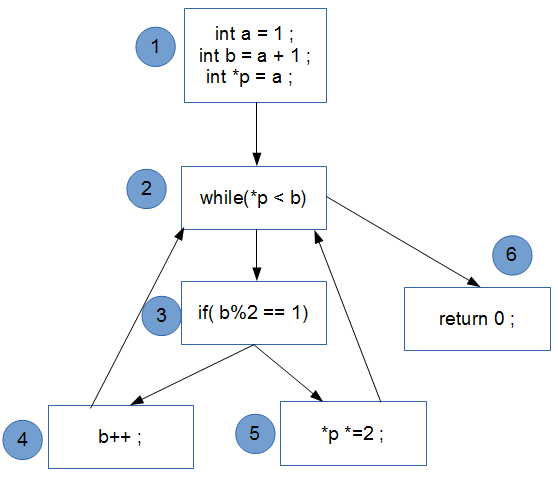
\includegraphics[scale=0.7]{soluce/CFG.jpg} 
	    \caption{CFG du code exemple}
	    \label{fig:CFG}
	  \end{figure}
	  
          Avec les informations obtenues pour ce graphe par C. Bacara,
          il est possible de modifier le graphe de flot de la manière
          suivante~:
	  \begin{figure}[H]
	    \centering
	    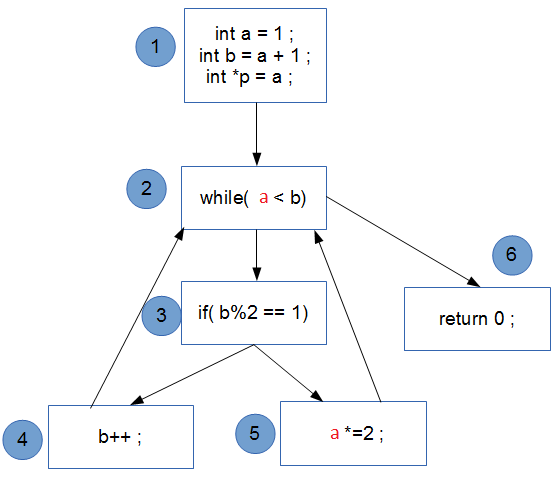
\includegraphics[scale=0.7]{soluce/CFGmodif.jpg} 
	    \caption{CFG du code exemple}
	    \label{fig:monlabl}
	  \end{figure}
	  
	  
	  Ainsi lors de la réécriture du programme, le code est modifié.
          Cette réécriture peut être effectué grâce à la classe Rewriter de LLVM qui permet grâce à des fonctions de haut niveau d'imprimer le CFG
          (\textit{insertText()},\textit{replaceText()}...).


      \subsubsection{La modification à l'impression du programme} 

	Elle consiste à parcourir le CFG, à récupérer les données (par
        exemple dans une matrice pour les alias (voir \ref{alias}) et ensuite faire les
        modifications lors de l'écriture du fichier sortie.

	C'est la méthode que j'ai choisie d'utiliser car elle est plus
        simple et rapide à mettre en oeuvre.
    


\section{Conclusion}

  LLVM est un outil très pratique à utiliser pour analyser un code source. 
  Grâce à ce framework et à une implémentation adaptée, on peut connaître les différentes propriétés d'un code C.
  
  Au cours de ce TER, j'ai pu mettre en oeuvre le cas d'un pointeur
  constant pour modifier les utilisations de ce pointeur dans le
  programme et ainsi permettre la suite des optimisations.
  Néanmoins l'algorithme permettant la modification des pointeurs n'a pas été implémenté.

  Lors de ce stage, j'ai pu découvrir le milieu de la recherche informatique, et j'ai beaucoup appris
  en terme de compilation avancée. De plus j'ai pu dévellopé mes compétences en C++ et j'ai découvert le framework LLVM
  qui pourra peut-être me servir plus tard.
\end{document}
